\section{GBM Design}
In this section, we will list the alternative loss functions and base learners, and explain when they can be used. Later, we will discuss some improvement approaches to GBM, such as combining different types of base learners, regularization, subsampling, and others. For more information about the design of GBM, we refer  to NateKin \cite{natekin2013gradient}.

To create a GBM for a particular task, it's important to choose the appropriate options for the empirical loss function $\mathcal{L}$ and the hypothesis $\mathcal{H}$ (which is the set of collections of base learners), because these choices have a significant impact on the GBM's performance. (As we discussed in the previous section, the conditional expectation function minimizes the $L^2$ loss.)


\subsection{Loss functions}
The loss function is a critical element of the gradient boosting machine, as it quantifies the discrepancy between the anticipated and actual values of the target variable. The selection of loss functions (functionals) depends on the objective of our model. For instance, if the goal is to obtain the conditional expectation of the response given $X$, the square loss function ($L^2$ loss) is preferable since the conditional expectation can be considered as the projection of the response, thus attaining the smallest $L^2$ distance to the response. To use a loss function in practice, one must specify both the loss and the corresponding negative gradient. (In our Python module, the loss function is defined as an abstract class with attributes "loss" and "negative gradient".) Other loss functions are provided in Schmid et al., 2011 \cite{schmid2011geoadditive}.

The types of loss functions can be roughly divided according to the type of response
as follows:
\begin{enumerate}
	\item \textbf{Continuous response:}
	\begin{itemize}
		\vspace{-.2cm}
		\item $L^2$ loss (Conditional Expectation)
		\vspace{-.2cm}
		\item $L^1$ loss (Conditional Median)
		\vspace{-.2cm}
		\item Quantile loss (Conditional Quantile)
		\vspace{-.2cm}
		\item ZeroOne loss (Conditional Mode).
		\vspace{-.2cm}
	\end{itemize}
	\item \textbf{Categorical response:}
	\begin{itemize}
		\vspace{-.2cm}
		\item Exponential loss
		\vspace{-.2cm}
		\item Cross-Entropy loss
		\vspace{-.2cm}
	\end{itemize}
	\item \textbf{Other response:}
	\begin{itemize}
		\vspace{-.2cm}
		\item MLE loss 
		\vspace{-.2cm}
		\item Custom loss
		\vspace{-.2cm}
	\end{itemize}
\end{enumerate}

%\begin{table}[htb]
%\centering
%\begin{tabular}{lcc}
%\toprule
%\textbf{Loss Function} & \textbf{Expression} & \textbf{Roles} \\
%\midrule
%$L^2$ Loss& $\frac{1}{2}(y-f)^2$ & conditional expectation \\
%ZeroOne Loss & $I\{y=f\}$ & conditional mode \\
%Exponential Loss & $\exp{(-yf)}$& weight redistribution \\
%CrossEntropy Loss& &   \\
%\bottomrule
%\end{tabular}
%\caption{Loss Functions}
%\label{tab:topmidbottom}
%\end{table}
The framework allows for the use of custom loss functions. One example of their application is in quantitative finance and investment analysis, particularly in stock selection. At each rebalance date, we have a multitude of factors denoted by $F_t \in \R^{m \times N}$, where $m$ is the number of factors and $N$ is the number of stocks. These factors include historical prices, financial ratios, and technical indicators. Our goal is to combine these factors into a vector $\alpha_t \in \R^N$ and then use a given strategy to obtain indicators like Sharpe ratio or excess alpha of future retures. This  can be viewed as a custom loss function.Specifically, we can represent the result at time $t$ as 
\begin{eqnarray*}
\mathrm{result}_t &=& \mathrm{Strategy}_t \circ f \circ F_t \\
 &=&\mathrm{Strategy}_t \circ \alpha_t.
\end{eqnarray*}
In this situation, the custom loss functional can be expressed as 
$$
\mathcal{L}: \mathcal{H} \to \R, \quad f \mapsto \frac{1}{T}\sum_{i=1}^T \mathrm{Strategy}_t \circ f \circ F_t.
$$
Here we use the $L^2$ loss function for illustration.

\begin{Theorem}{($L^2$ loss, general version)}\label{thm:gv} \ \\
Suppose $(\Omega, \mathcal{F}, P)$ is a probability space, $Y: \Omega \to \R$ and $X: \Omega \to \R^p$. The the solution of the following
$$
\argmin_{f \in \mathcal{H}} \Vert Y - f \circ X\Vert_2 ^2 =\argmin_{f \in \mathcal{H}} \int_{\Omega} (Y-f \circ X)^2 \D P
$$
is the function $m: \R^p \to \R, \quad x \mapsto E(Y|X=x).$
\end{Theorem}
Theorem \ref{thm:gv} provides ideas for choosing the loss function, but in practical applications, we also need to estimate based on the sample. Therefore, we propose the following method of converting from the population to the sample:
\begin{eqnarray*}
Y \in \mathcal{L}^1(\Omega) &\implies& (y_1,y_2,\cdots,y_n)^\prime \in \R^n. \\
f\circ X \in \mathcal{L}^1(\Omega) & \implies & (f(x_1), f(x_2), \cdots, f(x_n))^\prime \in \R^n.
\end{eqnarray*}
 that is, to use two vectors in $\R^n$ to approximate the distance between random variables.


\begin{Theorem}{($L^2$ loss, empirical version)} \ \\
Suppose $\mathcal{D}=\left\{ (y_i,x_i): i=1,2,\cdots,n \right\}$ is a sample from $(Y,X)$. Then the conditional expectation of $Y$ given $X$ can be approximated by 
$$
\argmin_{f \in \mathcal{H}} \frac{1}{2n} \sum_{i=1}^n (y_i - f(x_i))^2.
$$
\end{Theorem}

\subsection{Base Learners}
The base learn  also plays importtant roles in model design since the GBM can be seen as the linear combination of base learners. In this section, we will introduce some base estimators which was widely used in practice.

Initially, we define the base-learners as a group of functions that map $\R^p$ to $\R$. It is not necessary for it to be a Hilbert space, nor even a vector space. Therefore, we refer to it as a collection of functions instead of a function space. In practice, there are three types of base-learners.
\begin{table}[htb]
\centering
\begin{tabular}{lc}
\toprule
\textbf{Type} & \textbf{Base-Learner}  \\
\midrule
Linear models& Affine functions  \\
Smooth models & P-splines  \\
 & Kernel functions  \\
Decision trees & Decision tree  \\
\bottomrule
\end{tabular}
\caption{Base Learners}
\label{tab:base-learners}
\end{table}

Among the most prevalent base-learners are decision trees. Decision trees, regarded as simple-measurable functions, can approximate Borel-measurable functions in the $L^p$ norm, thereby demonstrating their universality. The decision tree algorithm operates by recursively partitioning the data into subsets based on the values of a specific input feature until a predetermined stopping criterion is fulfilled. The outcome is a tree-like structure, with each internal node representing a decision predicated on a feature's value, and each leaf node signifying a final decision or prediction.

Decision trees offer several advantages. They are straightforward to interpret and visualize, which aids in comprehending the decision-making process of a model. Additionally, they can handle both categorical and numerical data, making them versatile for different types of datasets, whether small or large.



\subsection{Combine different base learners}
In constructing a GBM model, the choice of base learners is not restricted, which allows for the incorporation of multiple classes of base learners simultaneously. Various studies have explored the selection of different types of base learners, including Generalized Linear Models (GLMs), Kernel functions, splines, among others. Some research efforts have even attempted to integrate diverse types of base learners within the boosting framework. For instance, studies by Sigrist \cite{sigrist2021ktboost} and Hoffmann \cite{hoffmann2004combining} achieved reduced bias and error by combining various types of base learners. We encapsulate these concepts in Algorithm 4.

\begin{center}
\begin{minipage}{0.95\linewidth}
\begin{algorithm}[H]
\setstretch{1.5}
\SetAlgoLined
\caption{The Combined Gradient boosting algorithm}
\KwData{$\mathcal{D}=\{(y_1,x_1),\cdots,(y_n,x_n)\}$}
\KwIn{\begin{itemize}
	\vspace{-.3cm}
	\item the hypothesis $\mathcal{H}_k$ and the reproducing kernel $K$.
	\vspace{-.3cm}
	\item the empirical loss function $\mathcal{L}: \mathcal{H} \to \R$
	\vspace{-.3cm}
	\item number of iterations $M \geq 1$
	\vspace{-.3cm}
	\item leanring rate $\eta \in (0,1]$
	\vspace{-.3cm}
\end{itemize}
}
Initialize $f_0, \quad f_0(x) = \argmin_{c \in \R} \frac{1}{n} \sum_{i=1}^nL(y_i,c)$ for all $x \in \R^p.$\\
\While{$m \in \{1,\cdots,M\}$}{
Calculate the negative gradient vector: 
\vspace{-.3cm}
$$
g_{m,j} = -\frac{1}{n}\sum_{i=1}^n \partial_2 L(y_i, f_{m-1}(x_i))K(x_i,x_j), \quad j = 1,2, \cdots, n.
\vspace{-.3cm}
$$ \\
\vspace{-.2cm}
Fit the gradient vector: 
$$
h_m^{(k)} = \argmin_{h \in \mathcal{H}_k,\beta} \sum_{i=1}^n (g_{m,i} - \beta h(x_i))^2
\vspace{-.2cm}
$$  \\
Find the best base learner and step size: 
\vspace{-.3cm}
$$
\rho_m, \ k^* = \argmin_{\rho, k} \mathcal{L}(f_{m-1} + \rho h_m^{(k)})
$$ \\
\vspace{-.5cm}
Update: $$f_m \gets f_{m-1} + \eta \rho_m h_m^{(k^*)}$$
}
\KwOut{$f_M = f_0 + \sum_{i=1}^M \eta \rho_m  h_m^{(k)}$}
\end{algorithm}
\end{minipage}
\end{center}
At each step, we use different types of learners to approximate the revised negative gradient vector. Then, in step 5, we choose the one that minimizes the empirical loss at this step. Finally, the output model is a linear combination of different types of base learners.



\subsection{Regularization}
\subsubsection{subsample}
Subsampling is a technique used in machine learning to improve the overall performance of models by reducing overfitting. This involves randomly selecting a subset of the training data for each iteration of the learning algorithm. By doing so, the variance of the model can be reduced, and it can prevent learning unnecessary noise in the data. The gradient descent algorithm based on subsample is commonly referred to as the stochastic descent algorithm (SGD). Empirical evidence has shown that the model trained by SGD often yields better results, which is presented in algorithm 5. Suppose we have M batches such that:
$$
\bigcup_{t=1}^M B_t = \{1,2,\cdots,n\}.
$$

\begin{center}
\begin{minipage}{0.95\linewidth}
\begin{algorithm}[H]
\setstretch{1.5}
\SetAlgoLined
\caption{The Revised Stochastic Gradient boosting algorithm}
\KwData{$\mathcal{D}=\{(y_1,x_1),\cdots,(y_n,x_n)\}$}
\KwIn{\begin{itemize}
	\vspace{-.3cm}
	\item the hypothesis $\mathcal{H}$ and the reproducing kernel $K$.
	\vspace{-.3cm}
	\item the empirical loss functional $\mathcal{L}: \mathcal{H} \to \R$
	\vspace{-.3cm}
	\item number of iterations $M \geq 1$
	\vspace{-.3cm}
	\item leanring rate $\eta \in (0,1]$
	\vspace{-.3cm}
	\item stochastic batches: $B_t, t=1,\cdots, M.$
	\vspace{-.3cm}
\end{itemize}
}
Initialize $f_0, \quad f_0(x) = \argmin_{c \in \R} \frac{1}{n} \sum_{i=1}^nL(y_i,c)$ for all $x \in \R^p.$\\
\While{$m \in \{1,\cdots,M\}$}{
Calculate the gradient vector: 
\vspace{-.3cm}
$$
g_{m,j} = -\frac{1}{|B_m|}\sum_{i\in B_m} \partial_2 L(y_i, f_{m-1}(x_i))K(x_i,x_j), \quad j \in B_m.
\vspace{-.3cm}
$$\\
Fit the gradient vector: 
$$
h_m = \argmin_{h \in \mathcal{H},\beta} \sum_{i\in B_m} (g_{m,i} - \beta h_m(x_i))^2
$$  \\
\vspace{-.3cm}
Find the best gradient descent step-size: 
\vspace{-.5cm}
$$
\rho_m = \argmin_{\rho \in \R} \mathcal{L}(\f_{m-1} + \rho h_m)
$$ \\
\vspace{-.5cm}
Update: $$f_m \gets f_{m-1} + \eta \rho_m h_m$$
}
\KwOut{$f_M = f_0 + \sum_{i=1}^M \eta \rho_m h_m$}
\end{algorithm}
\end{minipage}
\end{center}
The difference is that, we apply a stochastic batch $B_m$ to calculate the negative gradient.

\subsubsection{step size}
The step-size, or learning rate, is a critical hyperparameter in the gradient descent algorithm. It determines the magnitude of the update to the model parameters during each iteration. A large step-size can cause the algorithm to diverge, while a small step-size can result in slow convergence. The learning rate can also be thought of as the weight of the base learners. If the learning rate is too high, the algorithm will focus too much on the front part, which can reduce performance.
\subsection{RGBoost}
\begin{figure}[htb]
	\centering
	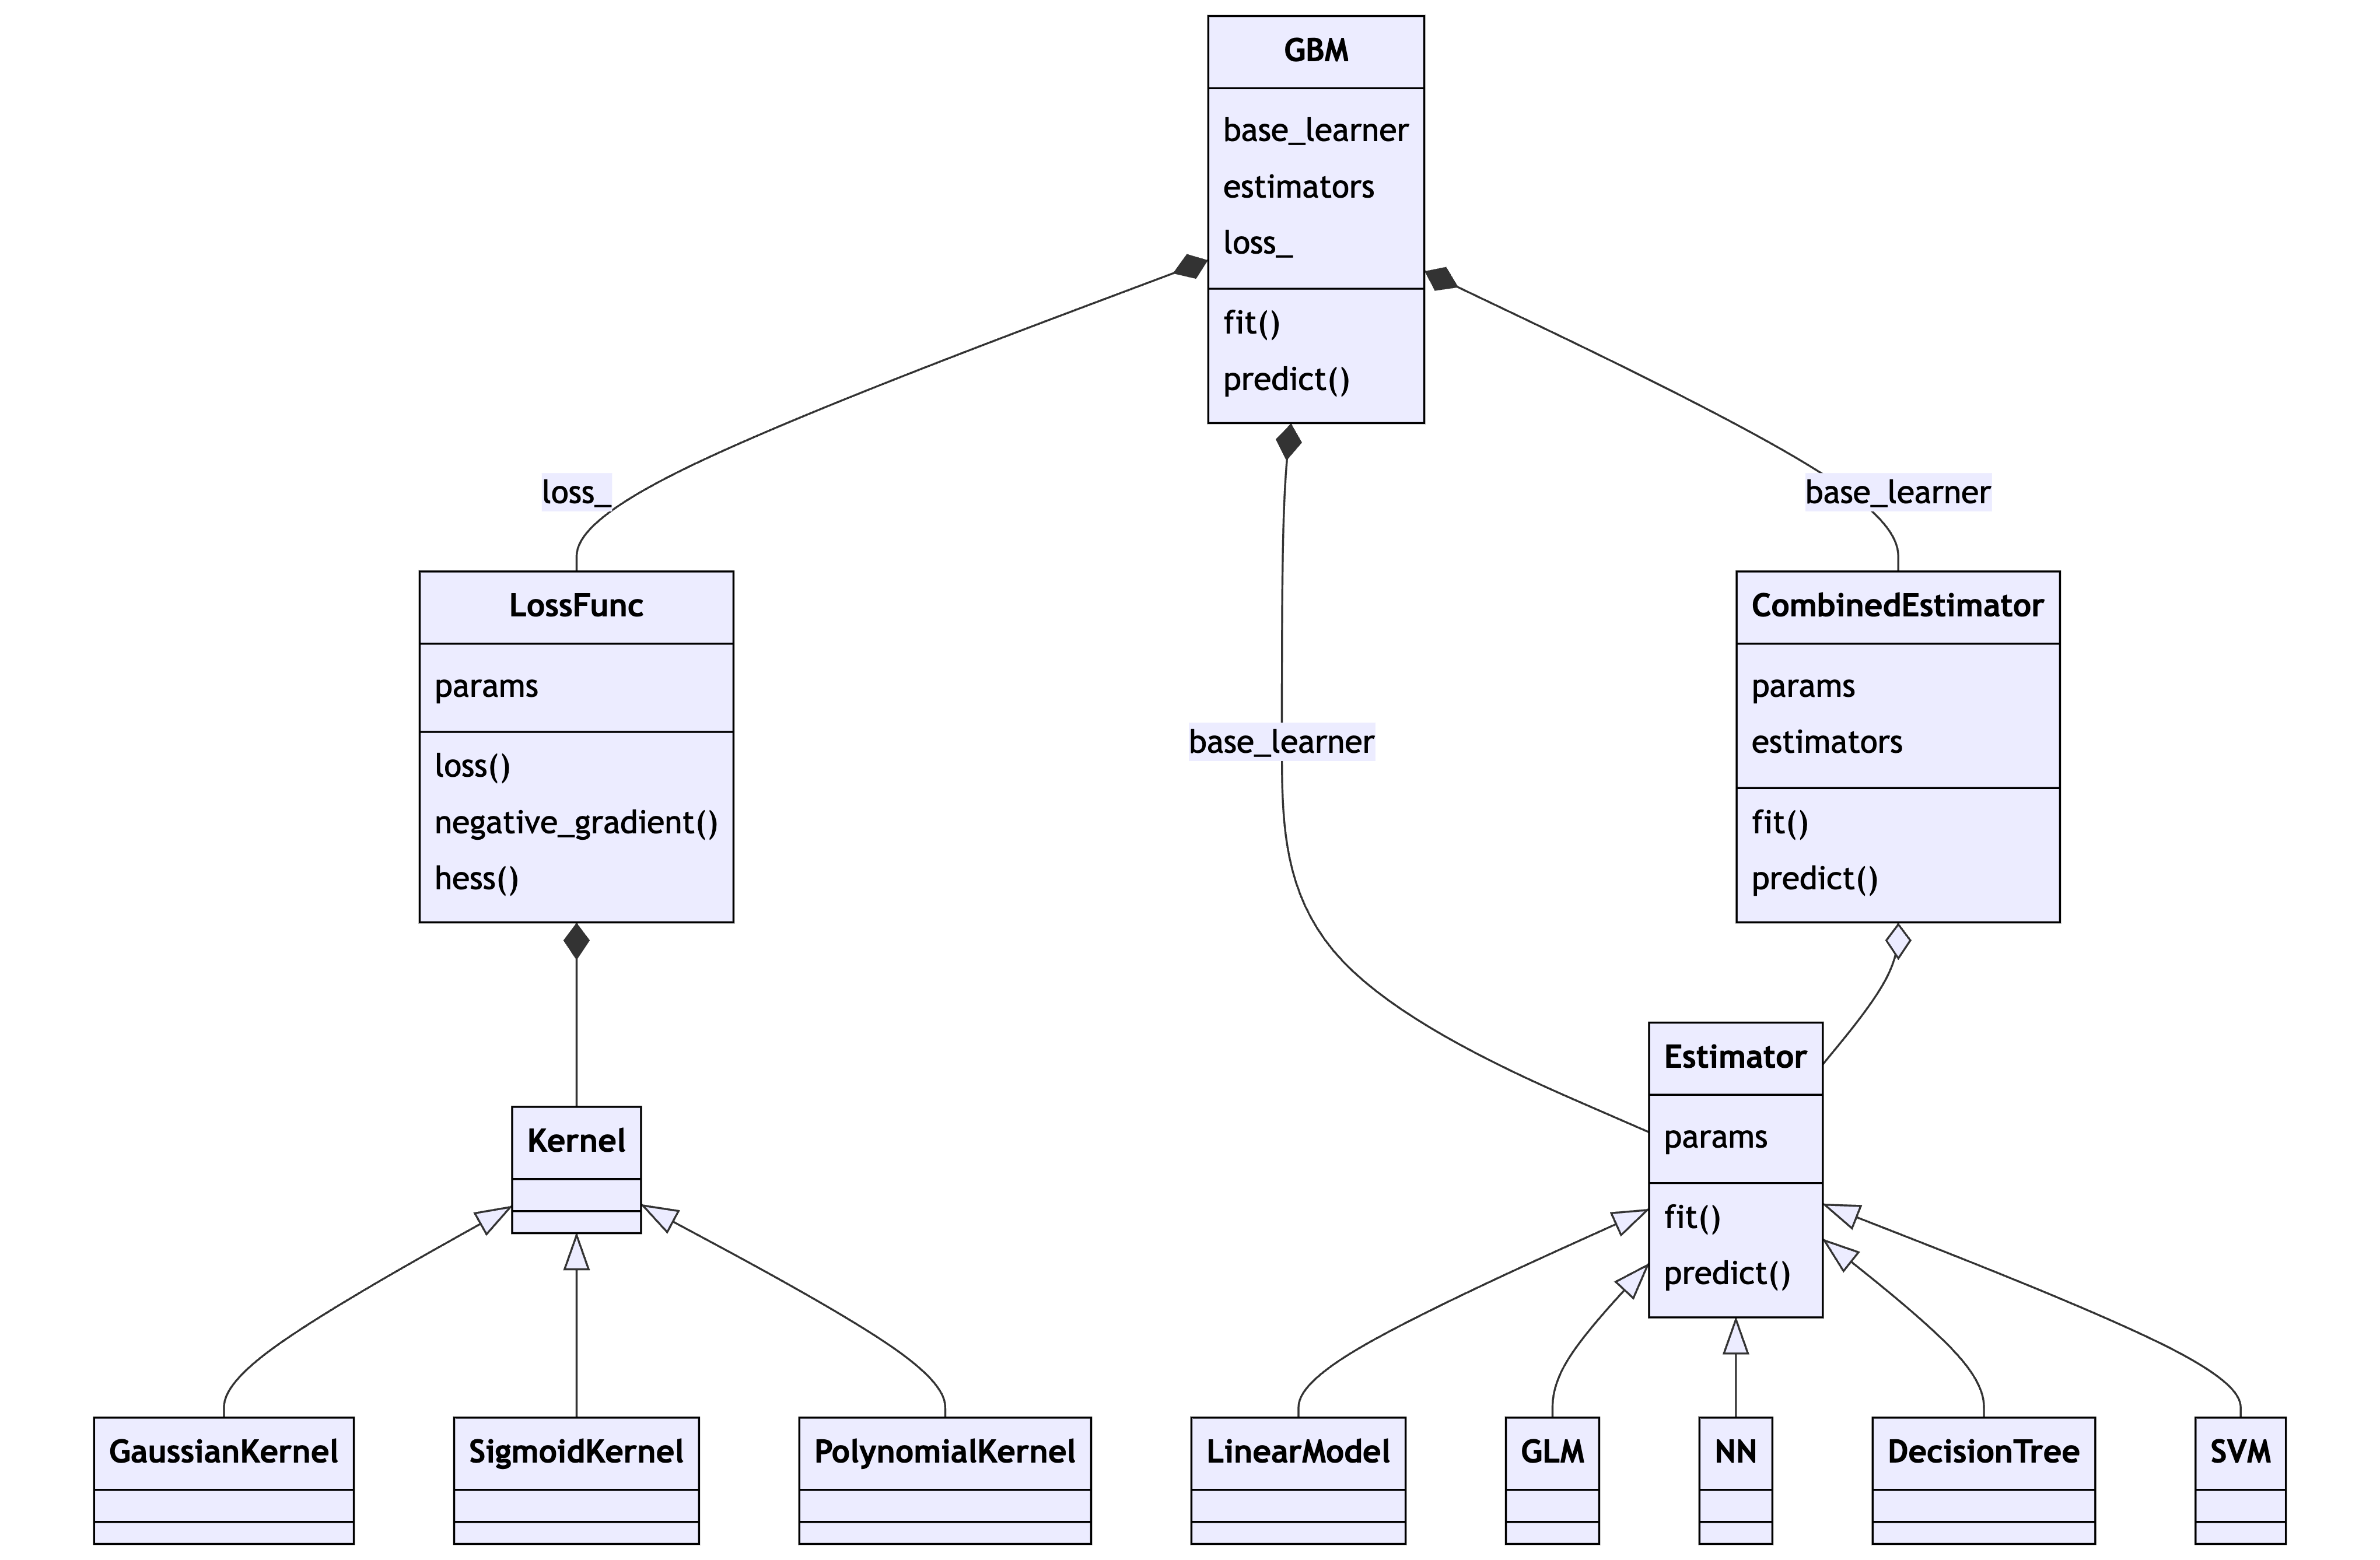
\includegraphics[height=10.5cm]{figure/rgboost.png}
	\caption{framework of rgboost}
\end{figure}
This subsection presents the RGBoost module\footnote{rgboost is available at https://github.com/nymath}. This module, based on the Python class GradientBoostingRegressor (Classifier) from the sklearn.ensemble package, is designed to yield consistent results. Unlike GradientBoostingRegressor, which restricts the base learner to decision trees, RGBoost supports the amalgamation of multiple base learners. This includes the combination function proposed by Sigrist\cite{sigrist2021ktboost}. Moreover, RGBoost integrates the gradient correction scheme proposed in this paper. One notable characteristic of our module is the versatility of the estimator class. In essence, any model with the "fit" and "negative gradient" attributes can serve as an estimator. This flexibility allows us to boost various models, such as neural networks, SVMs, GLMs, and even boosted models.Furthermore, we define the collections of different types of Estimator classes as a CombinedEstimator class. Similar to individual Estimator classes, the CombinedEstimator class also possesses "fit" and "negative gradient" attributes and, therefore, can be embedded within the GBM class.










